\chapter{Real-Life Measurements}
\label{sec:irl}

\section{Introduction}

In addition to theoretical results, real world cases must be measured
in order to validate the theory. In this chapter, methods for making actual
measurements in both snow and in engineered materials are explored. Moreover,
methods for building engineered materials are discussed.


\section{Needle Probe Measurement Fundamentals}

Needle probe measurements are taken using an apparatus borrowed from the Cold
Regions Research and Engineering Laboratory (CRREL), illustrated in Figure
\ref{fig:apparatus}. Encased in a Pelican case for protection are a Campbell
CR10X data logger, a relay switch, a 12v gel cell for the CR10X and a series of
D-cells to power the heating coils in the needle. The program that came with the
data logger uses the relay switch to control the heat flux from the needle, and
records temperature data from the needle's thermocouple, as well as the voltage
across the heating element, over the course of a five minute heating curve and
a ten minute cooling curve.

\begin{figure}[h]
\centering
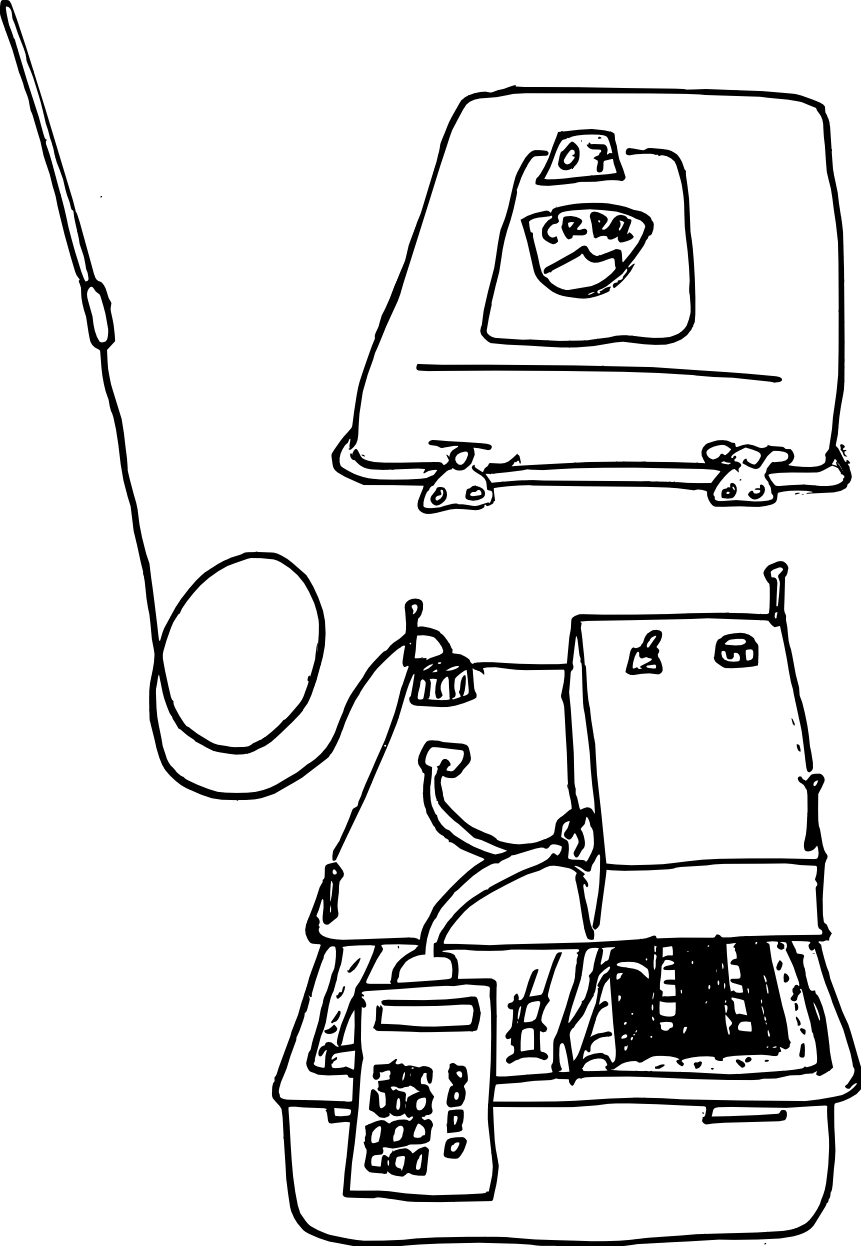
\includegraphics[width=0.7\textwidth]{fig/apparatus.png}
\caption{Extruded illustration of the needle probe apparatus. Major parts are labelled.}
\label{fig:apparatus}
\end{figure}

Once testing is complete, data may be uploaded from the data logger using
Campbell's PC200W software (shown in Figure \ref{fig:pc200w}) and a serial connection.

\begin{comment}
\begin{figure}[h]
\centering
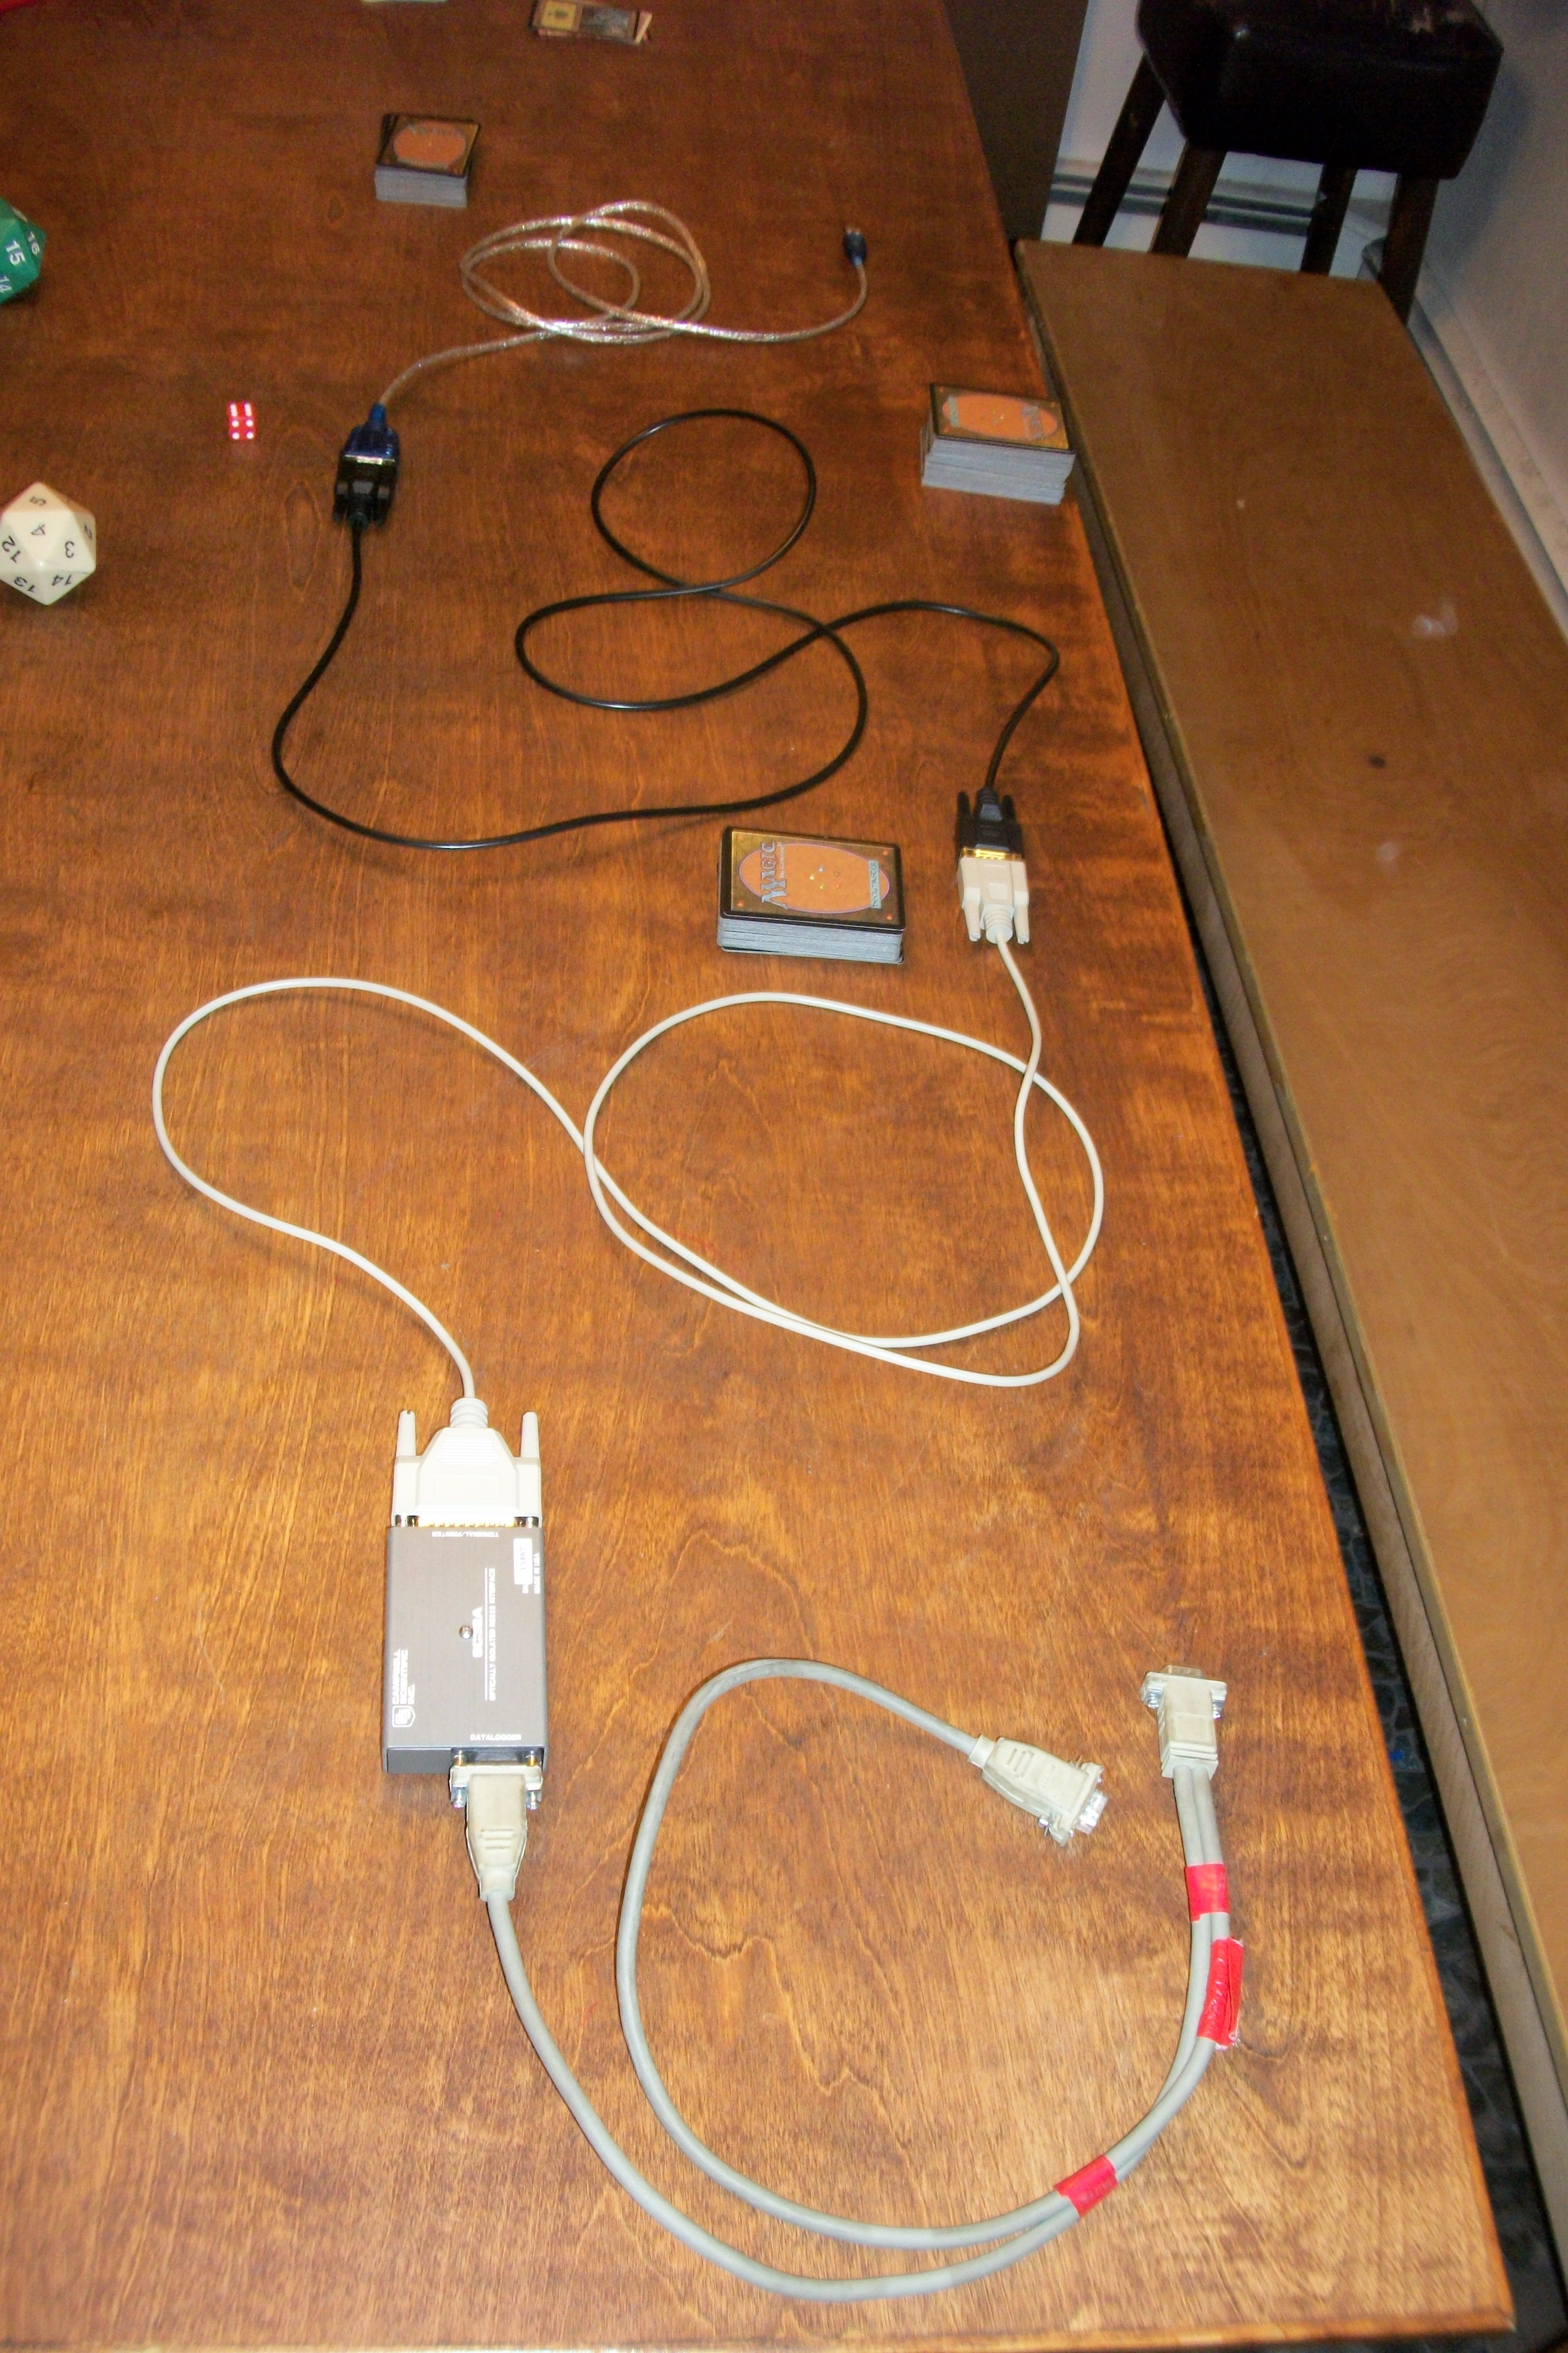
\includegraphics[width=0.6\textwidth]{fig/cable.jpg}
\caption{The cables used to communicate with the datalogger.}
\label{fig:cable}
\end{figure}
\end{comment}

Using PC200W, data may be uploaded from the CR10X in a raw binary format and then
converted to a .csv format. This .csv data may be analyzed with either spreadsheet software, a series of
scripts, or both. For this series of experiments, Excel, Gnumeric and cat/append are used
to verify the existence of data and to combine datasets, while python is used
for the analysis.  Generally, each analysis consists of subtracting \(t_0\)
from the relevant time intervals, subsetting the collected data over a straight
section, and finding the slope.  In addition, a correction factor, named the
McGaw Cooling Curve Correction after a CRREL researcher, is used for benchtop
measurements to account for the insulation around the apparatus.

Generally, each measurement also has some metadata associated with it. In
particular, anisotropic measurements have an angle associated with them, and
snow measurements also have a coordinate position on the snowpack associated
with them. These are measured with a protractor and a tape measure,
respectively. This means that, while taking measurements, one has to be careful
to make sure that they can keep the proper metadata associated with each
measurement.

\begin{figure}[h]
\centering
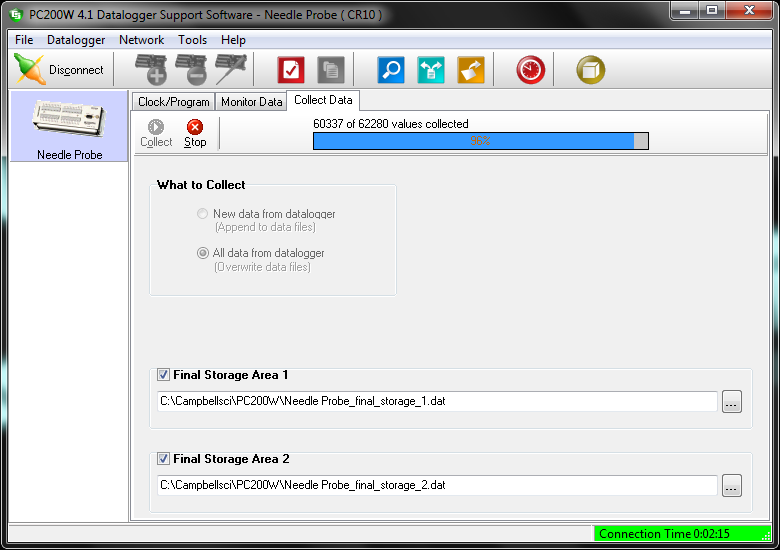
\includegraphics[width=0.8\textwidth]{fig/pc200w.png}
\caption{A screenshot of PC200W, the software used to pull data off the CR10X data logger.}
\label{fig:pc200w}
\end{figure}

Unlike the case of numerical experiments, it is extremely important in
real-world experiments---especially in the case of snow---to hand-inspect every
time/temperature curve. This is because, unlike the numerical experiments, there
is a significant chance that data will not be usable. In the case of snow in
particular, convection is typically experienced near the end of the heating
curve and the beginning of the cooling curve.

\begin{figure}[h]
\centering
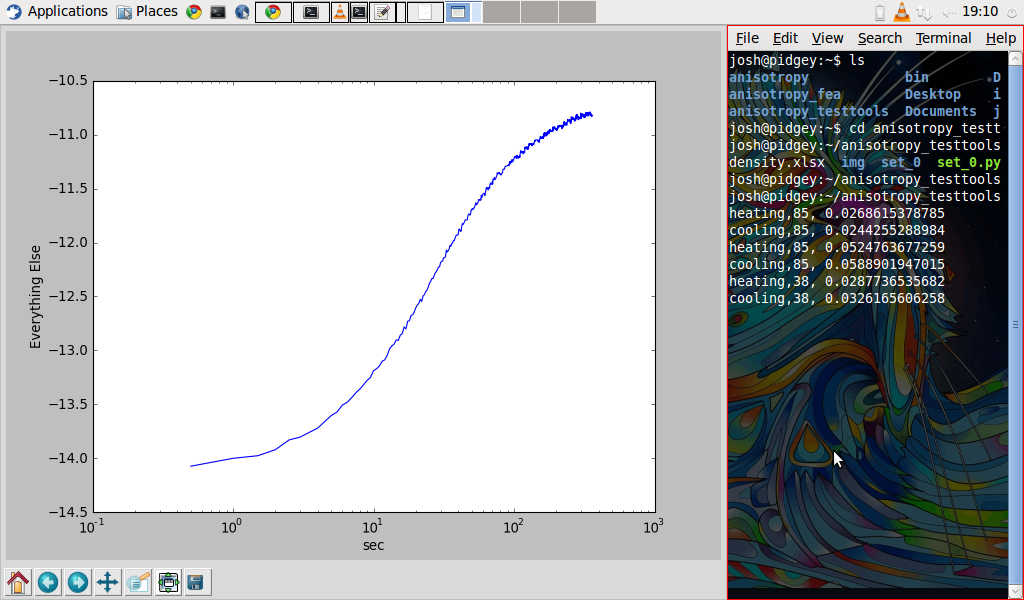
\includegraphics[width=0.8\textwidth]{fig/measurement_graph.png}
\caption{A plot of temperature vs. time from a real-world measurement of snow.
Each curve must be analyzed by-hand to check for such effects as convection, as seen on the right-hand side of this curve.}
\label{fig:meas_graph}
\end{figure}



\section{Snow Conductivity Measurements}

The first step in measuring proper snow is to make a vertical cut in the
snowpack, as in Figure \ref{fig:snowpack}.

\begin{figure}[h]
\centering
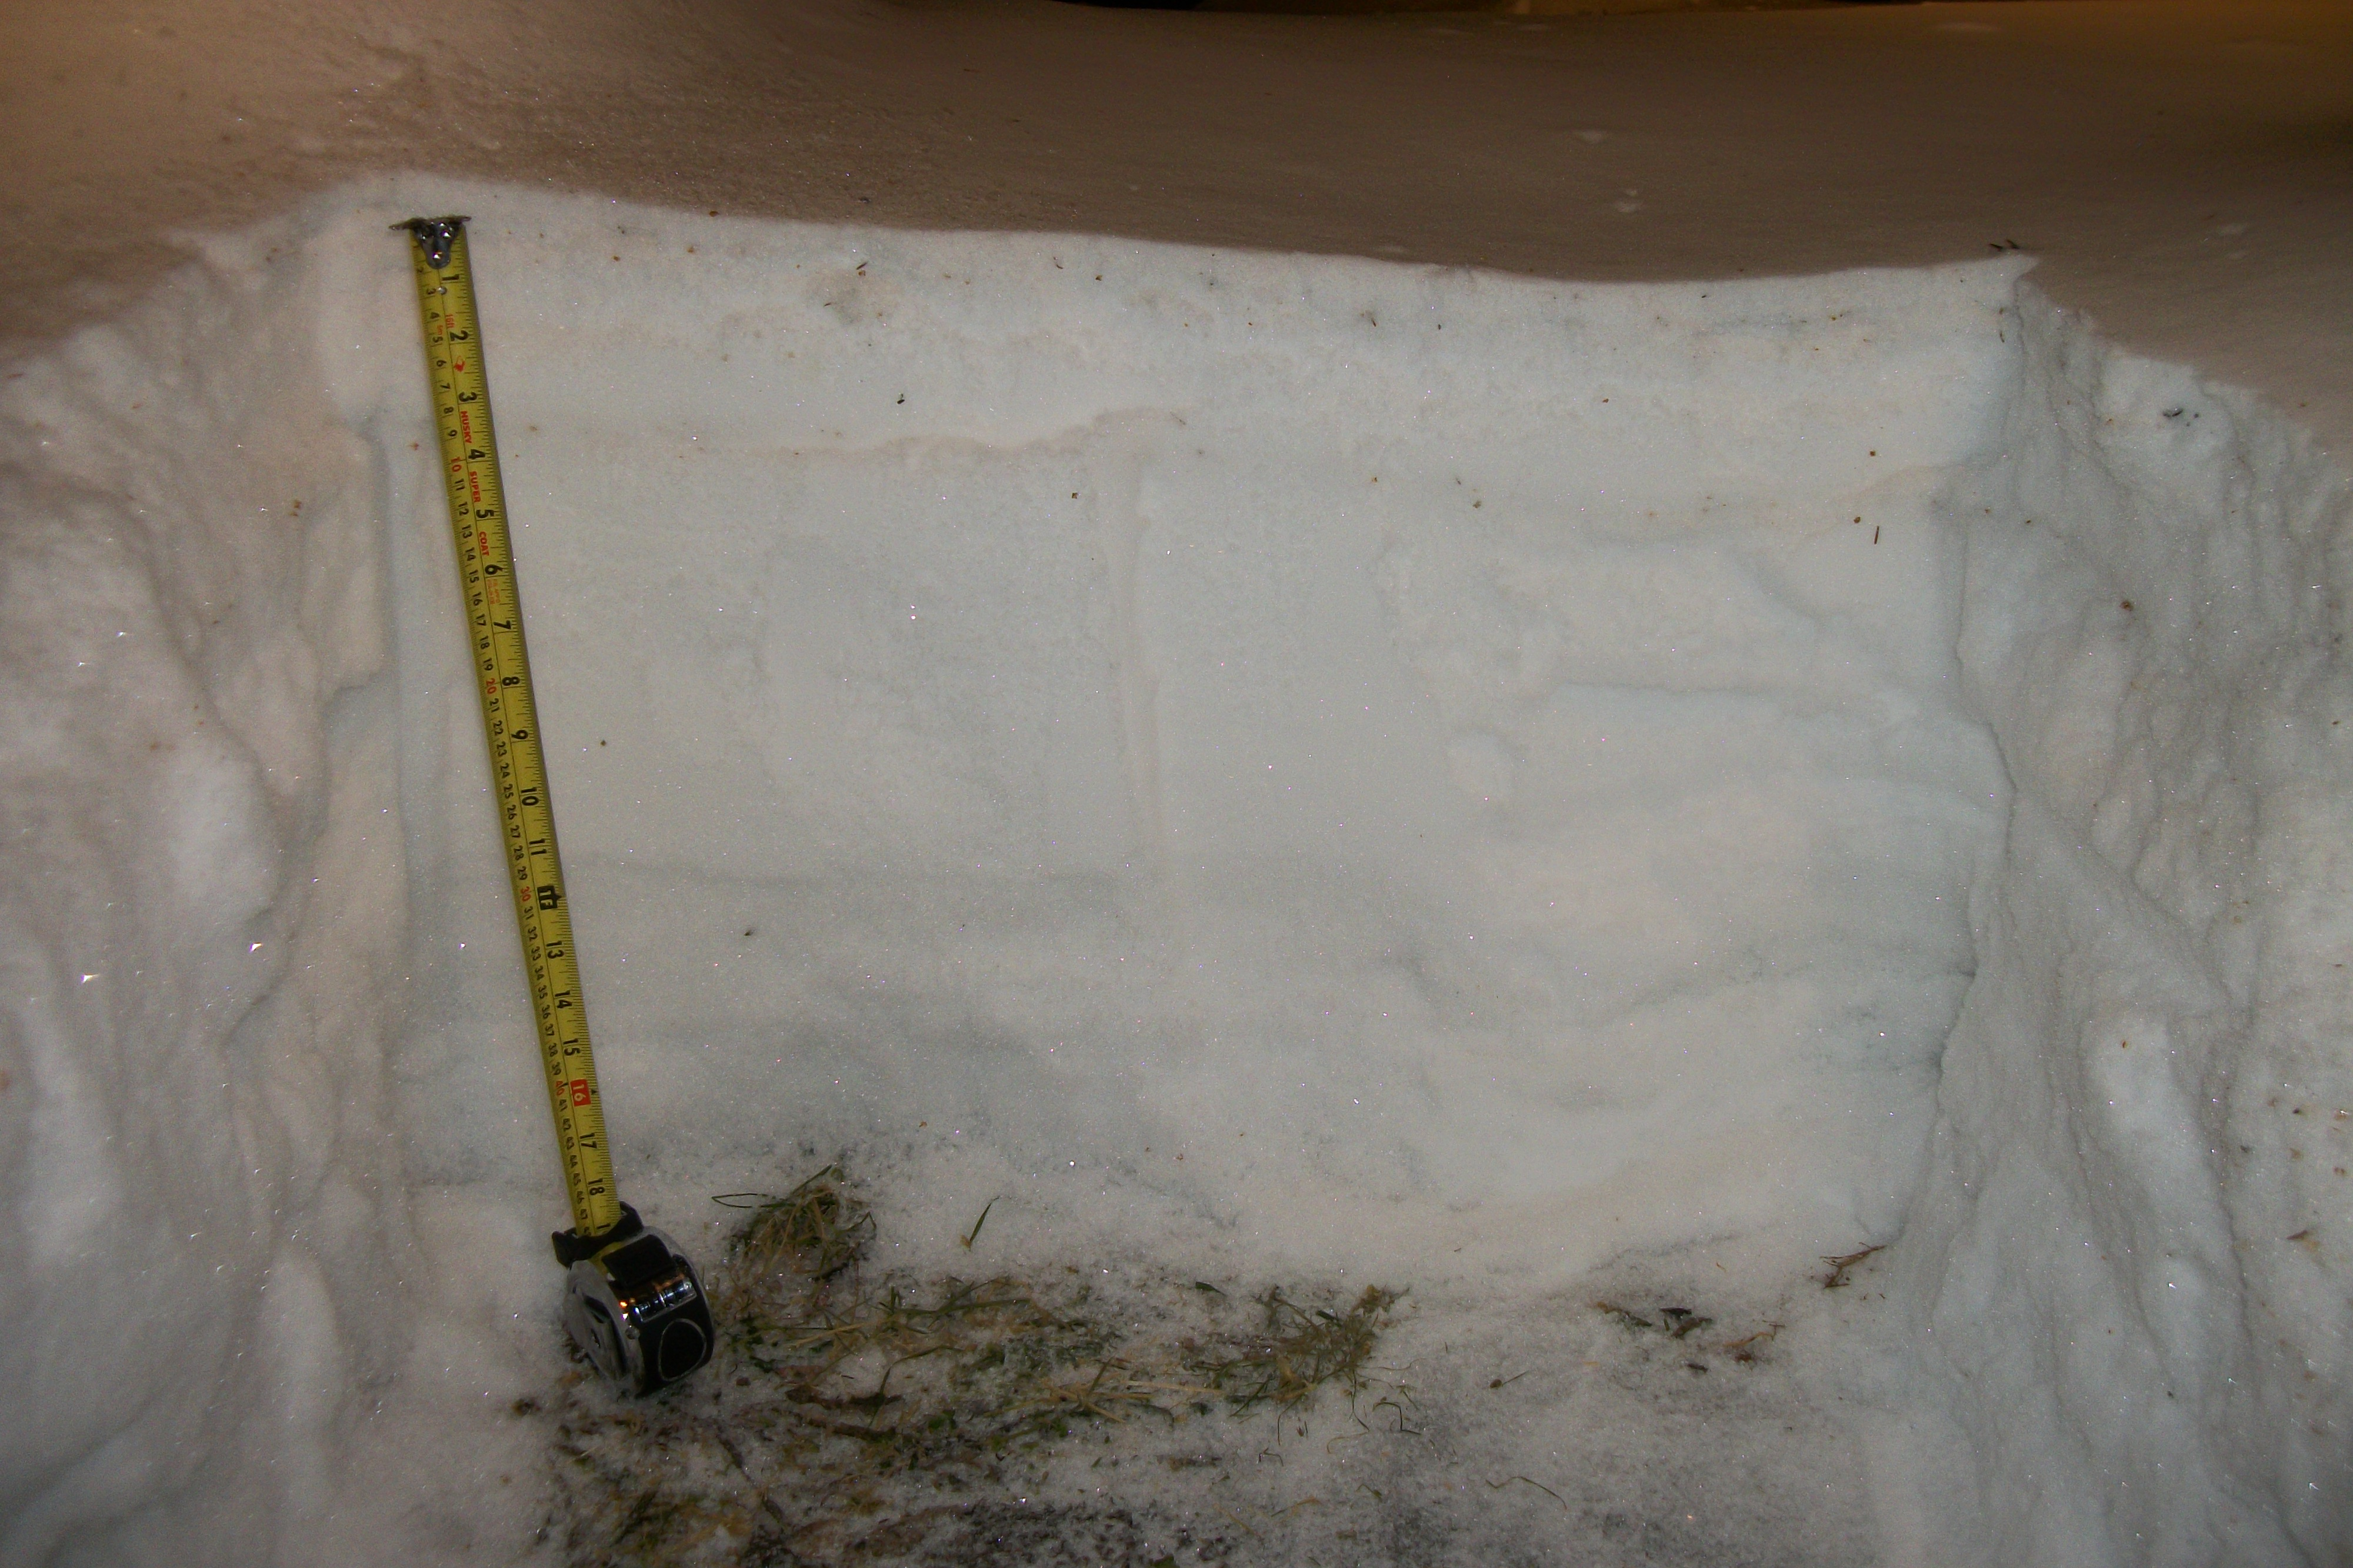
\includegraphics[width=0.8\textwidth]{fig/snowpack.jpg}
\caption{A close-up shot of tested snowpack.}
\label{fig:snowpack}
\end{figure}

Then, for every measurement, the needle is inserted into snow and a measurement
is taken. Snow is relatively difficult to work with due to the low structural 
integrity of the material.  The wire connecting the probe to the data logger is
stiff enough at low temperatures that situating the needle without ruining the
snowpack can be quite a challenge.

Along with each conductivity measurement, the height from the ground---measured
with a tape measure---and the angle of insertion---measured with a protractor
and a plumb bob---were recorded as metadata.In addition, for each series of measurements at a particular region, the density
of the snow is also measured with a cardboard cylinder (used as a control volume)
and a scale.

\begin{comment}
\begin{figure}[h]
\centering
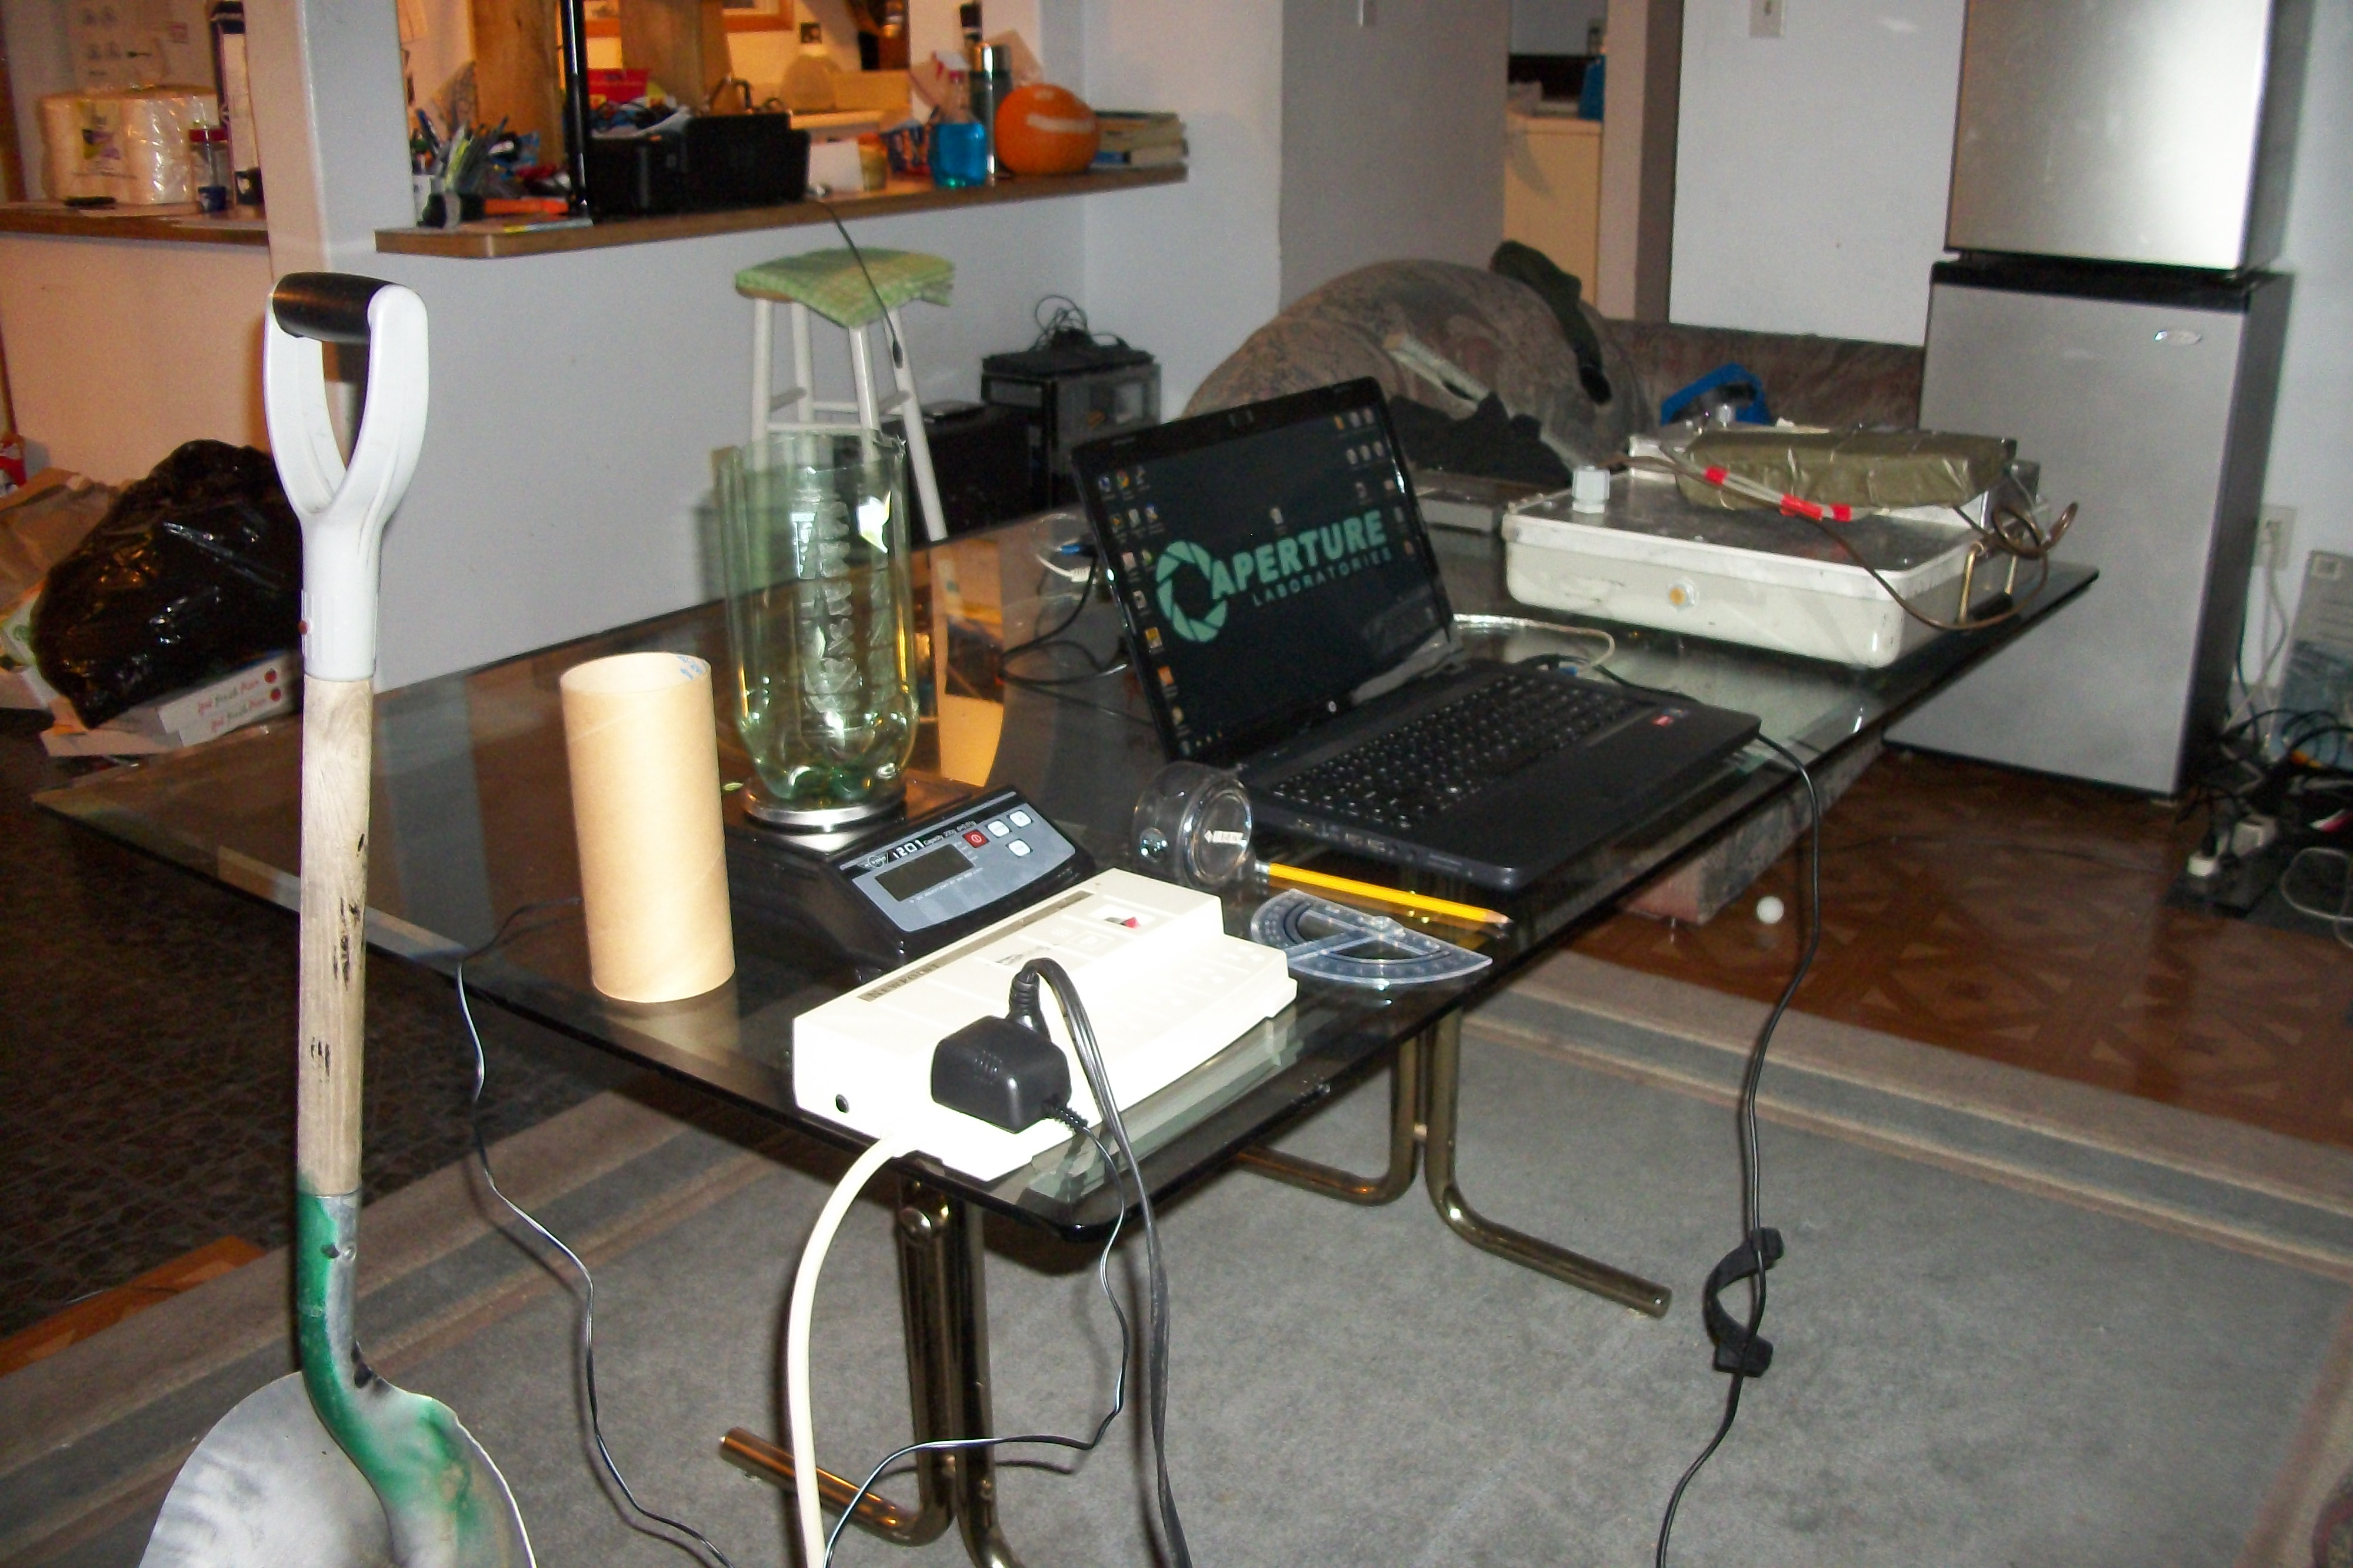
\includegraphics[width=0.8\textwidth]{fig/equipment.jpg}
\caption{Equipment used to measure snow thermal conductivity.}
\label{fig:equipment}
\end{figure}
\end{comment}

\begin{comment}
\begin{figure}[h]
\centering
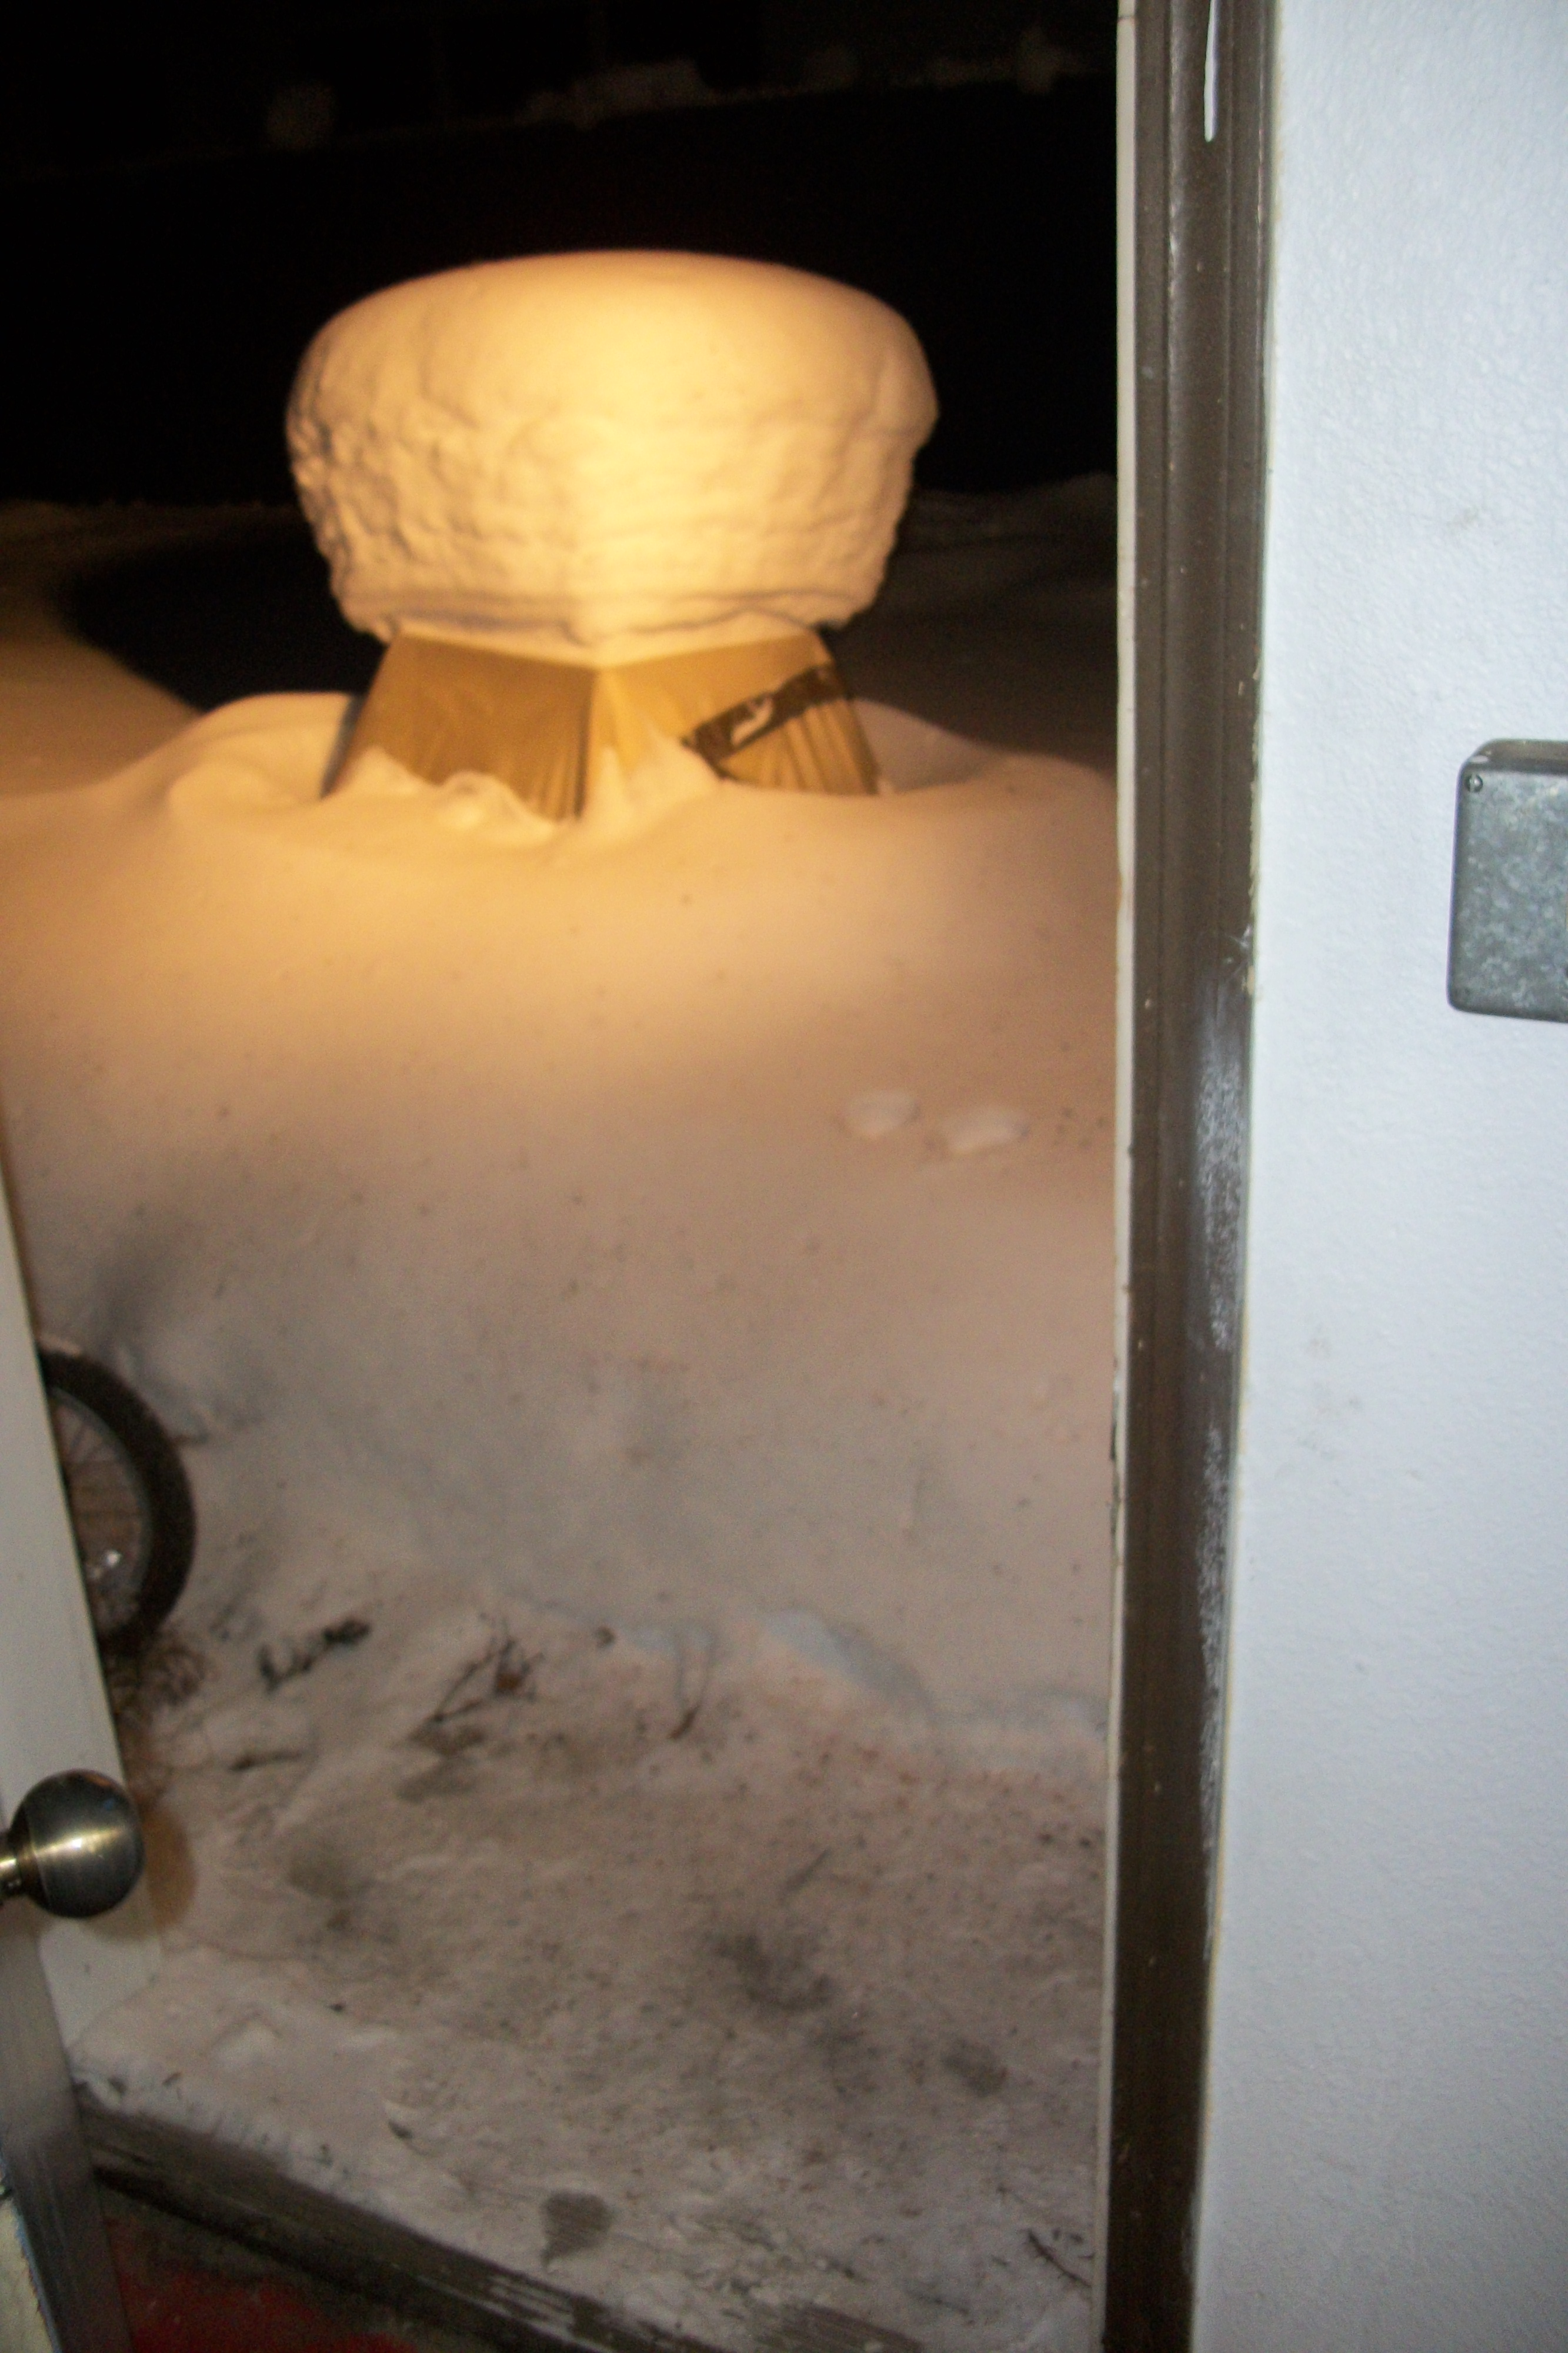
\includegraphics[width=0.4\textwidth]{fig/insitu_location.jpg}
\label{fig:insitu_location}
\caption{The location for in-situ tests.}
\end{figure}
\end{comment}

\section{Benchtop Tests}

A standard used to benchmark needle probes is to measure the conductivity of a
large Nalgene bottle full of glycerine and surrounded in insulating foam to
mitigate changes in room temperature. Glycerine was chosen because, while it
should have the same conductivity of water, does not readily convect. Moreover,
glycerine does not leave an air gap between the needle and the surrounding
medium like many porous materials, such as snow, will.

A method for testing anisotropic measurements by using alternating alternating
layers of more-conductive and less-conductive materials has been devised, based on
this glycerine benchmark test. However, instead of glycerine, the materials
used are table salt and table sugar.

\section{Raw Materials for the Anisotropic Composite}

Salt and sugar's conductivities alone were both measured using the needle probe
apparatus. These measurements resulted in conductivities of
\(0.225\) \(\textrm{W}/\textrm{m}/\textrm{K}\) and 
\(0.106\) \(\textrm{W}/\textrm{m}/\textrm{K}\), respectively.

\begin{table}[h]
\centering
\begin{tabular}{l l | l l | l l}
Material & \# & Heating & Cooling & Average & Standard Deviation\\
Pure salt & 1 & 0.222 & 0.220 & 0.225 & 0.015\\
 & 2 & 0.218 & 0.256 &  & \\
 & 3 & 0.216 & 0.219 &  & \\
Pure sugar & 1 & 0.108 & 0.113 & 0.106 & 0.008\\
 & 2 & 0.098 & 0.109 &  & \\
 & 3 & 0.094 & 0.113 &  & \\
\end{tabular}

\caption{Raw results of salt and sugar measurements after calculating conductivity. The multiple results were averaged for the purpose of predicting anisotropic conductivity of an alternately-layered medium.}
\label{tab:saltnsugar}
\end{table}

Assuming alternating layers of equal thickness, the anisotropic thermal
conductivities in the aggregate should be:

\begin{align}
k_{xy} &= \frac12 \left( k_{\textrm{salt}} + k_{\textrm{sugar}} \right) &= \boxed{0.166}\\
k_z &= 2 \left( \frac1{k_{\textrm{salt}}} + \frac1{k_{\textrm{sugar}}} \right)^{-1} &= \boxed{0.144}\\
\frac{k_z}{k_{xy}} &= \boxed{0.870}
\end{align}

Despite the conductivity of table salt being roughly twice that of sugar, the
anisotropic conductivity ratio is fairly close to one, meaning that the anisotropy
of the experimental medium, while significant, is relatively weak. Advantageously, however, salt and sugar are relatively inexpensive media to work with.

\section{Apparatus for Containing Anisotropic Composite}

\begin{figure}[h]
\centering
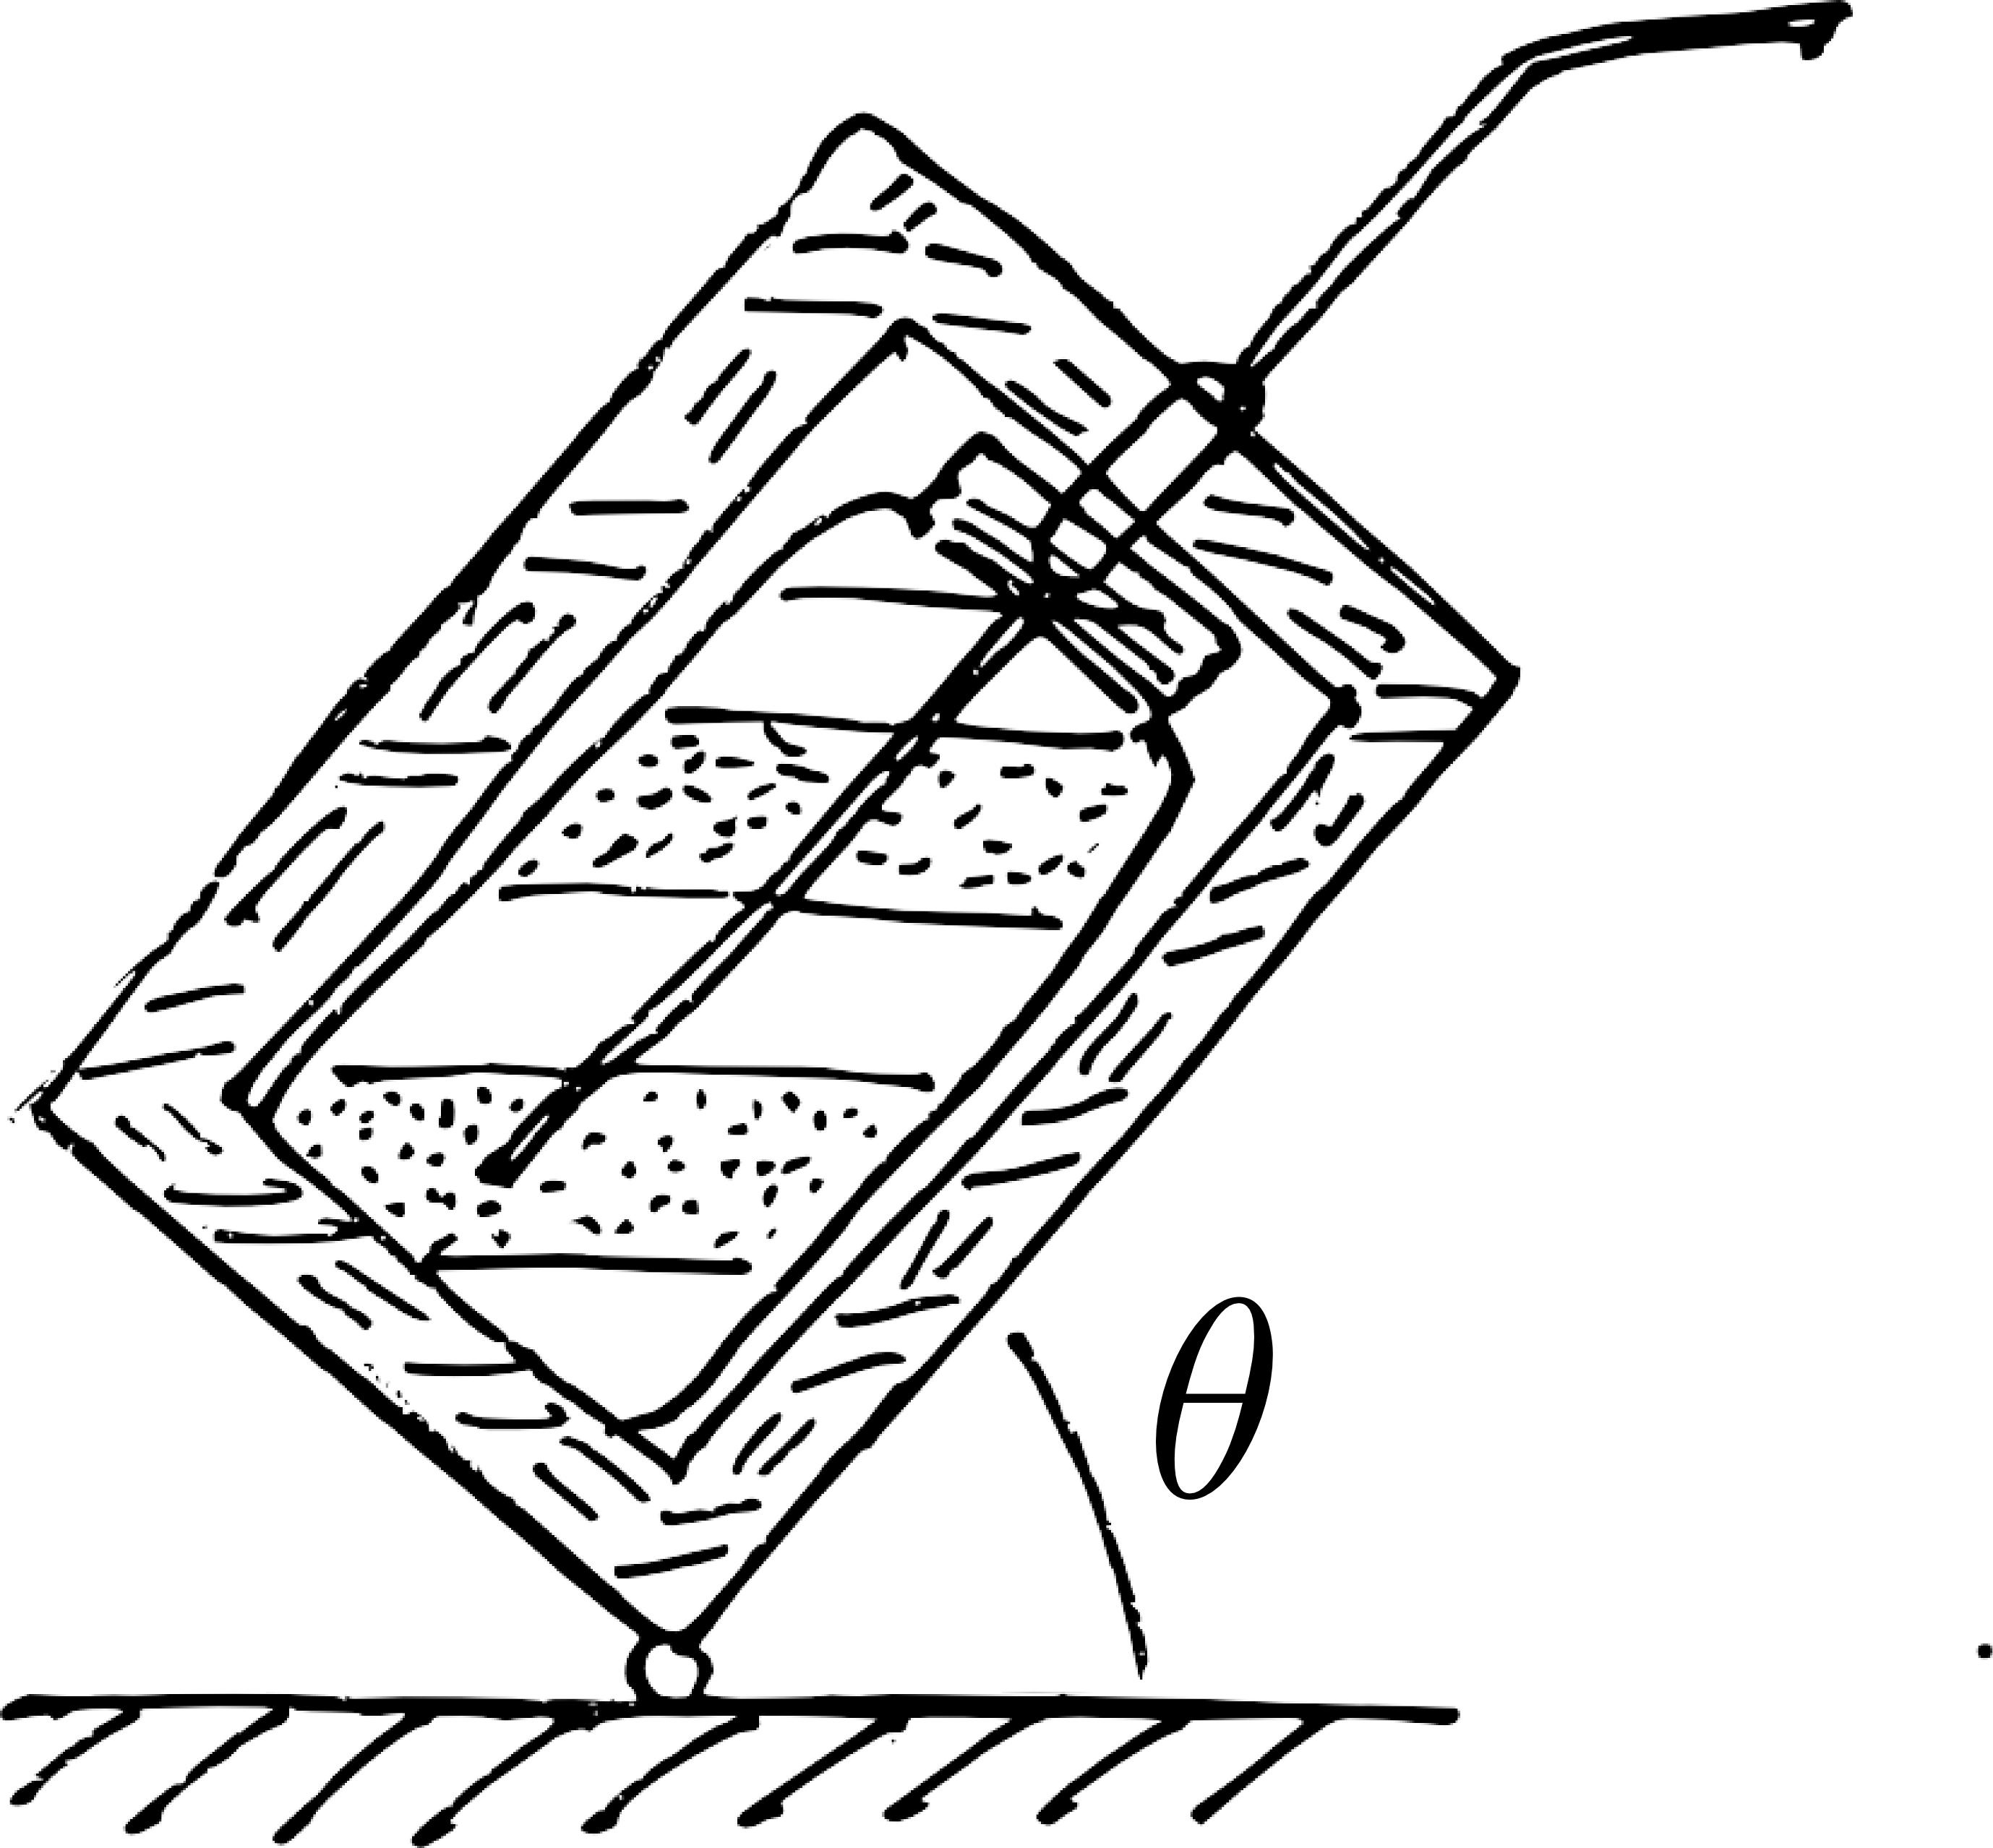
\includegraphics[width=0.4\textwidth]{fig/tilter_diagram.png}
\caption{An illustration of the apparatus used in benchtop measurements. The
apparatus was designed to tilt in order to cause alternating layers of self-
leveling materials to meet the needle at a given angle. However, the materials
actually used were not self-leveling, meaning the tilting apparatus was of 
limited utility.}
\label{fig:tilter_diagram}
\end{figure}

In order to effectively change the directions of anisotropy, a foam box for the
nalgene bottle was built that could be rotated on an axis and clamped in place.
The resulting angle from the horizontal can be measured with a protractor. The apparatus was designed with gels such as glycerine in mind, such that the layers
would self-level. However, because powders were used instead of gels, leveling
had to be done by hand, usually with a spoon. The sugar was dyed green in order
 to differentiate it from the salt.

\begin{figure}[h]
\centering
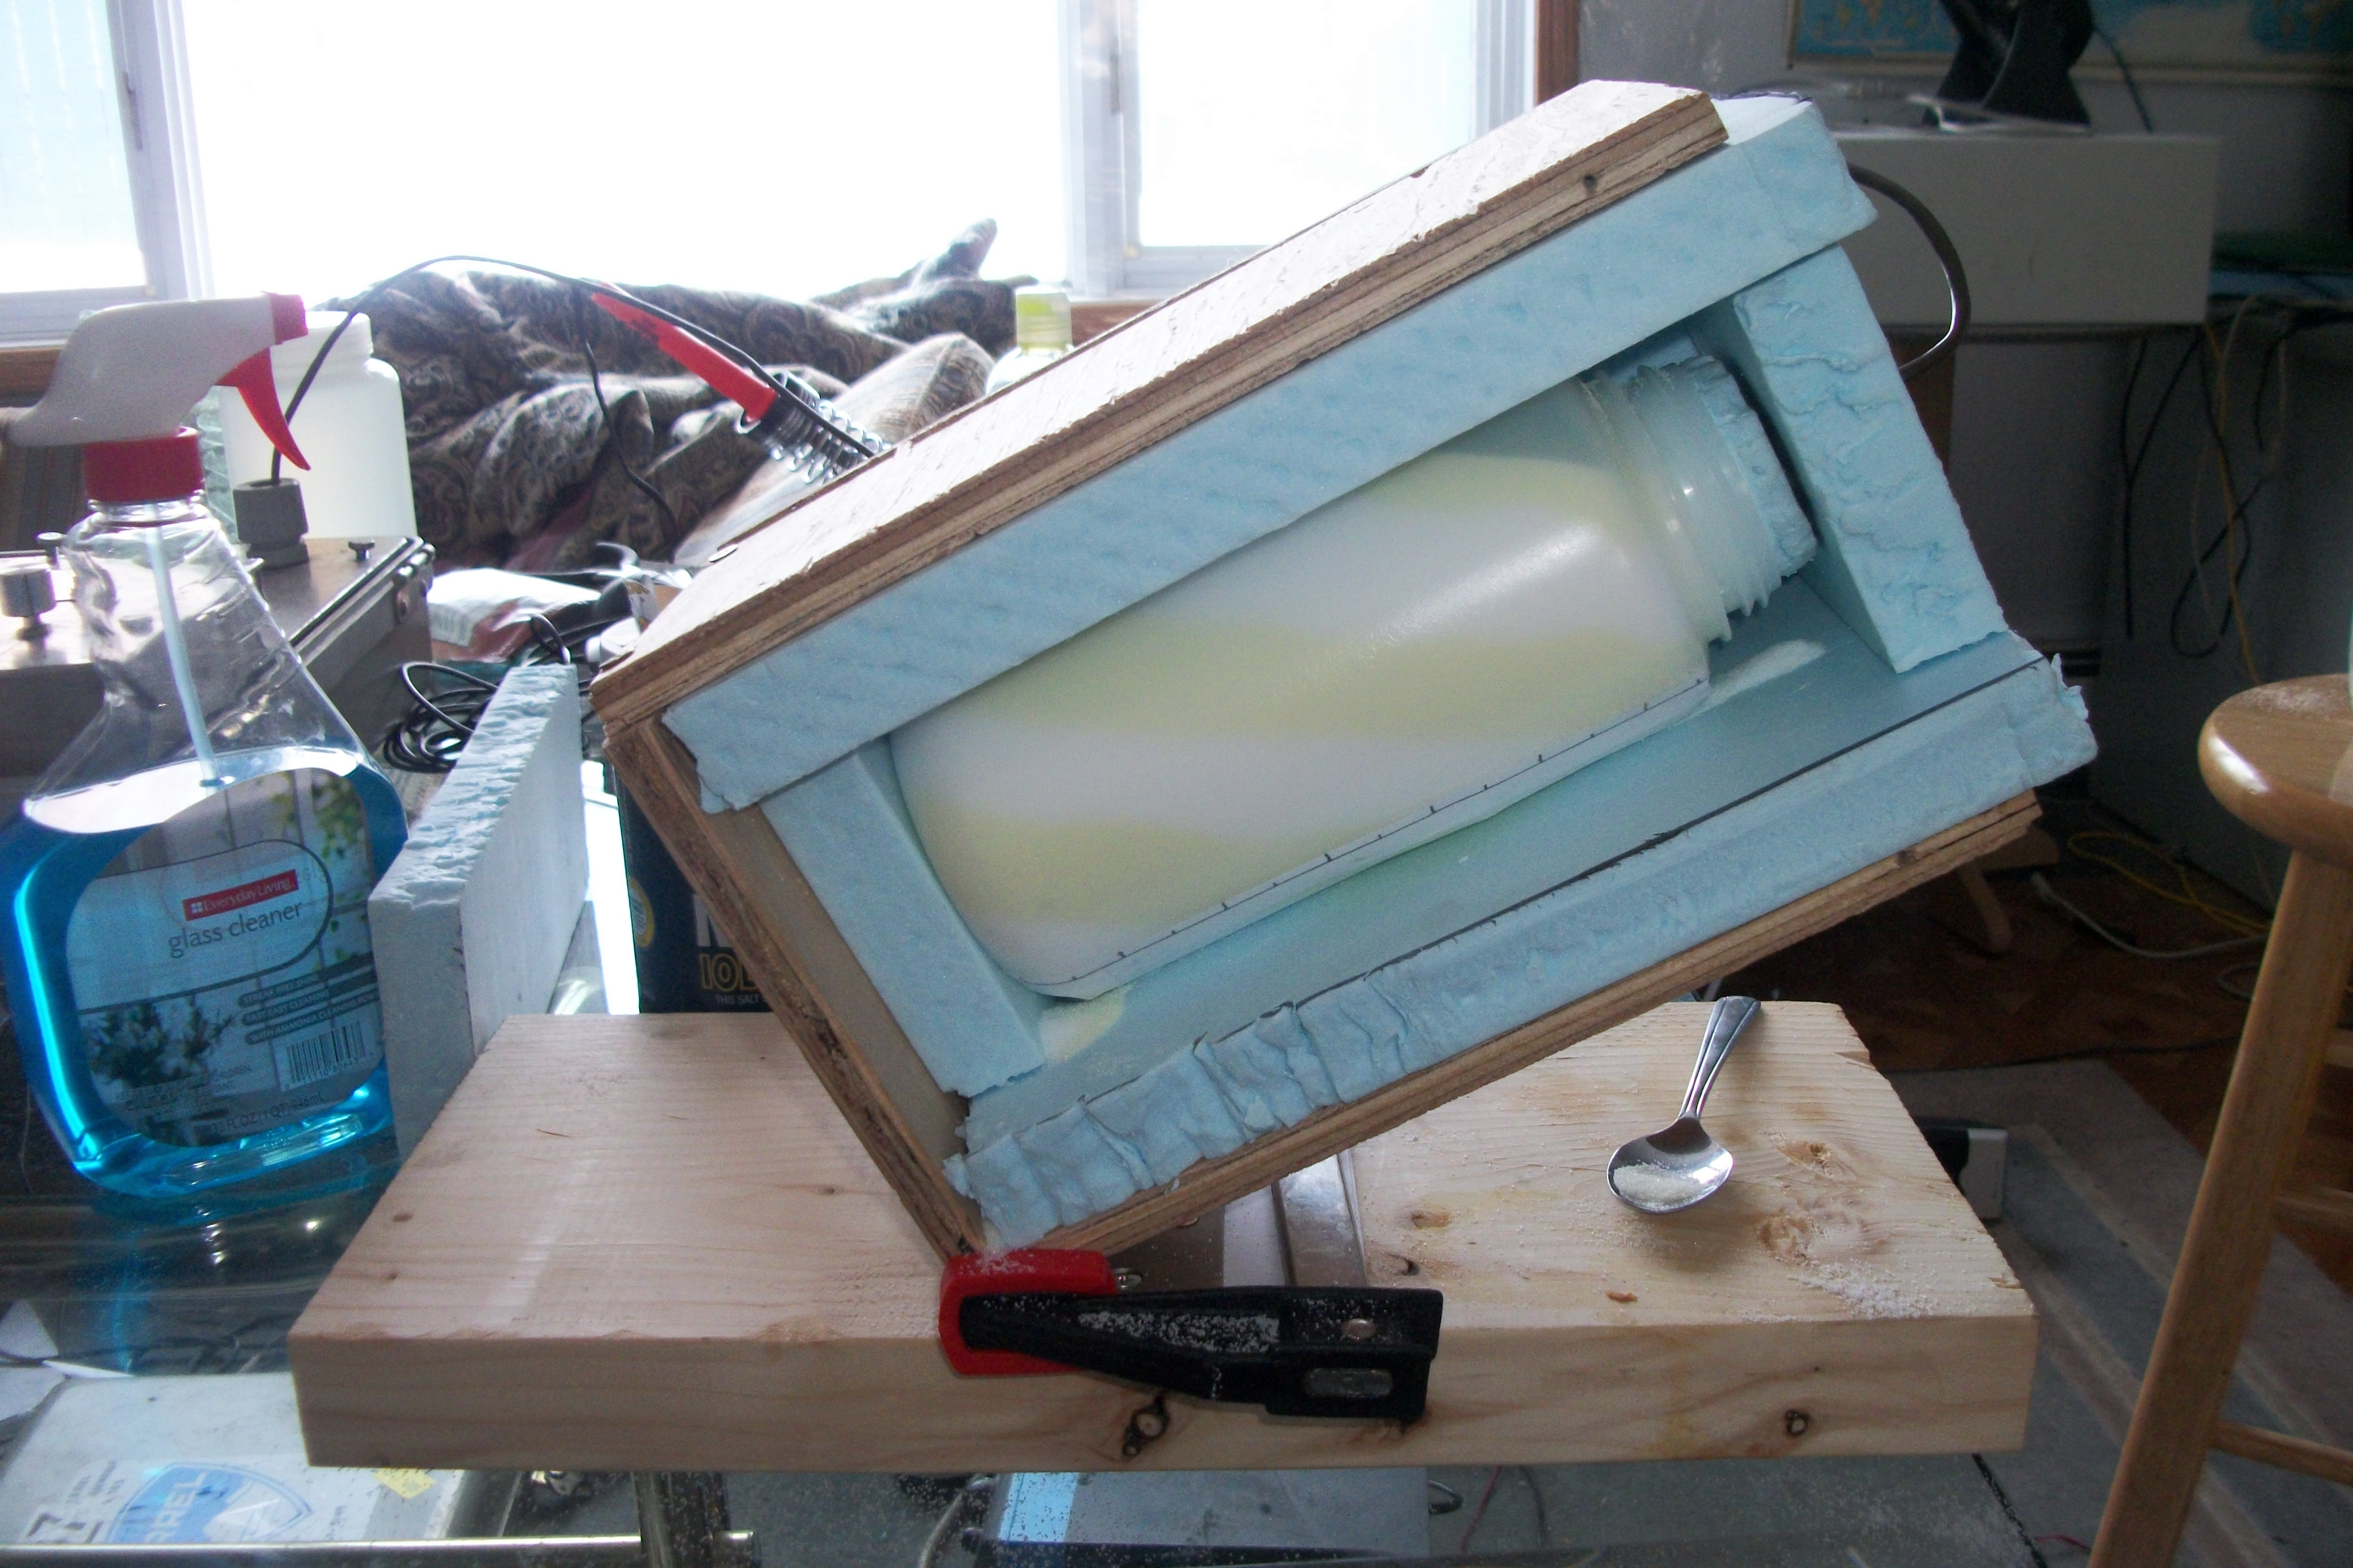
\includegraphics[width=0.6\textwidth]{fig/tilter_irl.jpg}
\caption{A photograph of the benchtop measurement apparatus in use, at 30 degrees.}
\label{fig:tilter}
\end{figure}
